\documentclass{article}
\usepackage[utf8]{inputenc}
\usepackage[spanish]{babel}
\usepackage{graphicx}
\usepackage{verbatim}
\usepackage{moreverb}
\usepackage{amsmath}
\usepackage{mathtools}
\usepackage{amsfonts}
\usepackage{amssymb}
\usepackage{fancybox}
\usepackage{float}
\usepackage{fancyvrb}
\usepackage{color}
\usepackage{url}
\usepackage{multicol}
\usepackage{tikz}
\usepackage[a4paper, hmargin=2cm, vmargin=2.5cm]{geometry}

%Nuevo comando: Inserta una línea recta.
\newcommand{\HRule}{\rule{\linewidth}{0.5mm}}

\begin{document}

%%%%%%%%%%%%%%%%%%%%%%%%%%%%%%%%% PORTADA %%%%%%%%%%%%%%%%%%%%%%%%%%%%%%%%%%%%%%

\begin{center}

{ \huge \bfseries Un sistema de comunicaciones}\\[0.4cm]

\large Julián Gutiérrez (51141) |
\large Pablo Pauli (51185) |
\large Ivan Itzcovich (53891) |
\large Gustavo Del Giudice (51289)\\[0.3cm] 

\end{center}

%%%%%%%%%%%%%%%%%%%%%%%%%%%%%%%%%%%%%%%%%%%%%%%%%%%%%%%%%%%%%%%%%%%%%%%%%%%%%%%%

% Seteo marcos para lo que esté en el entorno verbatim
\fvset{frame=single}

\begin{abstract}
\par Un sistema de comunicaciones establece un medio por el cual se envía y se recibe un mensaje a través de un canal. El usuario de este sistema de comunicaciones espera, aún desconociendo el mecanismo de transmisión que el mensaje transmitido sea exactamente idéntico al que lo recibe. Para esto, el canal debe mantener la identidad del mensaje y conservar su estructura, de otra manera el mensaje se vería modificado, y en consecuencia, el receptor estaría adquiriendo un mensaje distinto al original. Esta situación es imposible de lograr, puesto que un canal, al ser un medio físico, impone ciertas modificaciones al mensaje que está viajando por él. Estas modificaciones se deben a un comportamiento propio del canal, como por ejemplo la resistencia de los materiales del canal o la irrupción del medio en el cual habita el canal, el cual es imposible ignorar. En particular, en este trabajo se analiza el caso de un canal de índole informático, en el cual viajan datos digitales por un sistema de comunicación discreto en banda base.
\par El objetivo principal es poder desarrollar un sistema que, a partir de un mensaje recibido, se pueda revertir el problema que ocasionarán las modificaciones que le imprime el canal; para luego, una vez que se conoce dicho comportamiento, poder reinterpretar un mensaje recibido para obtener el mensaje original que fue enviado.
\end{abstract}

\begin{multicols}{2}

\section{Introducción}


\par Un modelo muy simple de un sistema de comunicaciones consiste de un transmisor que envía un dato cada cierto tiempo.Los datos son modificados por el canal, es decir, por el medio donde son transmitidos.Esta modificacion se genera por la respuesta al impulso del
canal. Además de ser modificados por el canal, los datos son afectados por ruido blanco Gaussiano aditivo. Teniendo en cuenta estas modificaciones, el receptor obtiene una respuesta.
\par Lo que nos interesa es, usando la respuesta que obtiene el receptor, conseguir la señal que se envió al inicio de la comunicación. El problema es que las modificaciones al canal y la longitud de la respuesta al impulso no suelen ser conocidas, por lo tanto debemos estimarlos. 
Si la longitud es conocida, es posible estimar la respuesta al impulso del canal mediante cuadrados minimos. Para esto, hay que enviar una señal conocida por el receptor. La denominamos secuencia de entrenamiento.Luego, se estima el canal planteando otro problema de cuadrados minimos. 
\par A continuación, se va a detallar la metodología con la que se realizó el trabajo, para luego exponer los resultados que se obtuvieron al realizar las distintas pruebas que requería el mismo, seguido de las conclusiones obtenidas.

\section{Metodología}
\subsection{Modelado}
\label{sec1}

\par El mensaje se transmite por un transmisor, el cual envía un dato del mensaje cada cierto intervalo de tiempo. Si el mensaje es $s_{k}$, entonces $s_{0}$ es enviado en t=0, $s_{0}$ en $t$=$T$ , $s_{2}$ en $t$=$2T$ ,etc. Cada dato transmitido es modificado por el canal como respuesta al impulso que genera el mismo. Esta modificación se puede presentar como $h_{k}$ (con $k$=$0$ a $L$), donde $L$ es la longitud de la respuesta al impulso. Además, los datos son perturbados con ruido blanco Gaussiano aditivo, $N_{k} \sim \mathcal{N} (m,\sigma)$.

\par La ecuación del dato recibido responde entonces a la siguiente:
\begin{equation}
\label{eq1}
r_{n} = \sum_{k=0}^{L-1} h_{k} s_{n-k}+N_{n}
\end{equation}
\par Esta ecuación se expresa de forma matricial como:
\begin{equation}
\label{eq2}
\vec{r} = H\vec{s}+\vec{N}
\end{equation}
\par Donde r es el mensaje recibido, compuesto por los datos recibidos; s es el mensaje transmitido, N es el ruido blanco Gaussiano, y H es la matriz de toeplitz, que corresponde a las modificaciones que se establecen en el mensaje transmitido, de tamaño MxM (siendo M la cantidad de datos que posee el mensaje a transmitir).
\par La ecuación (2) se puede expresar también de la siguiente manera:
\begin{equation}
\label{eq3}
\vec{r} = S\vec{h}+\vec{N}
\end{equation}

\par Manteniendo r y s equivalentes, siendo S la matriz toeplitz del dato transmitido y h el vector de la perturbación del impulso del canal.

\subsection{Inicializando y Perturbando}
\label{sec2}


\par En primer lugar, fue necesario simular el vector $h$, es decir, la respuesta al impulso del canal que se genera el transmitir el mensaje.  Para esto, se consideró $L$=$5$, y luego el $h$ se lo obtuvo a través de un una simulasion pseudo-aleatoria con distribución normal. La variable $\sigma$, fue inicializada en 0,01. Para obtener $H$,matriz de toeplitz que luego se va a utilizar para simular la transmisión, se utilizó la función “toeplitz” de Octave. Esto se puede observar en el código de “initializeCannal.m” del anexo. Vale destacar la ya mencionada matriz $H$ cumple la siguiente propiedad:
\begin{equation}
\forall \quad a_{i,j} \in H \to a_{i,j}=a_{i+1,j+1}
\end{equation}
%\begin{equation}% \label{tMat1}%
%\mathbf{H} = 
 %\begin{bmatrix}
  %\mathbf{h}_{0} & \mathbf{0} & \mathbf{0} &\cdots & \mathbf{0} & \mathbf{0}&\cdots & \mathbf{0} & \mathbf{0} \\
 % \mathbf{h}_{1} & \mathbf{h}_{0} & \mathbf{0} &\cdots & \mathbf{0} & \mathbf{0}&\cdots & \mathbf{0} & \mathbf{0} \\  
 % \ddots & \ddots & \ddots &\ddots & \mathbf{0} & \mathbf{0}&\cdots & \mathbf{0} & \mathbf{0} \\
  
  %  \mathbf{h}_{L-1} & \mathbf{h}_{L-2} &\cdots & \mathbf{h}_{1} & \mathbf{h}_{0} & \mathbf{0}& \cdots & \mathbf{0} & \mathbf{0} \\
  %  \mathbf{0} & \mathbf{h}_{L-1} &\cdots & \mathbf{h}_{2}  & \mathbf{h}_{1}& \mathbf{h}_{0} & \cdots & \mathbf{0} & \mathbf{0} \\
   % \ddots & \ddots & \ddots & \ddots & \ddots & \ddots & \ddots & \ddots & \ddots \\
  %\mathbf{0} & \mathbf{0} &  \mathbf{0} &  \mathbf{0} &  \mathbf{0} &  \mathbf{0} &  \cdots & \mathbf{h}_{1}& \mathbf{h}_{0} 
 %\end{bmatrix} \\
 %\in \mathbb{R}^{M \times M}
%\end{equation}

\par Con el h establecido, que de ahora en adelante va a ser referido como h “real”, se puede simular la transmisión de un mensaje. 
\par El objetivo principal del trabajo es el de “revertir el problema que ocasionan las modificaciones que le imprime el canal", tal como dice el Resumen. Para realizarlo, se tomo como mensaje a perturbar (y luego a reinterpretar),  la famosa imagen de “Lena”:
\begin{figure}[H]
\centering
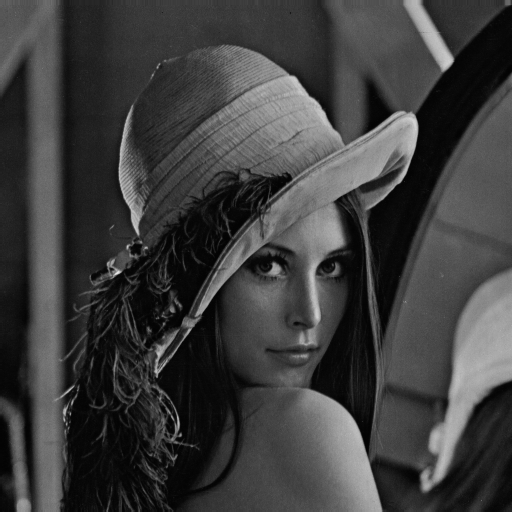
\includegraphics[scale=0.2]{../img/lena512.png}
\caption{Imagen 512}
\label{Imagen 512}
\end{figure}
\par Esta imagen sirve como imagen de prueba para los algoritmos de compresión de imagen, se lo considera un estándar científico. La imagen se transmite por filas por conveniencia, es decir, que nuestro dato sk es la fila k de la imagen. Para la transmision, se usa la ecuacion (2) del Modelado, por cada fila que se transmite. Es decir, fue necesario realizar un loop iterando sobre todas las filas de la imagen para perturbarlas. Dicho proceso se incluye en el ciclo “for” de “simulation.m” del anexo. Es importante mencionar que en este mismo ciclo se realiza la tarea de reinterpretación, que se explica más adelante. En la sección Resultados, se puede apreciar las modificaciones que sufre “Lena” al pasar por el canal de transmisión. También es importante aclarar que se realizaron múltiples recuperaciones de imágenes, variando ciertos parámetros que más adelante se detallarán, y para cada una de estas se simuló la transmisión, obteniéndose así múltiples imagenes recibidas.
\par Otra aclaración importante, visible claramente en el código, que es importante resaltar es que por un tema de eficiencia, para disminuir la cantidad de operaciones que debe realizar el Octave para operar con los vectores, cada fila que se envía (y luego se reinterpreta) es transmitida por partes, exactamente en 16 (esta modificación permitió que el tiempo que lleva cada iteración por fila bajara notablemente).  


\subsection{Estimando h}
\label{sec3}

\par Para lograr el objetivo de revertir las modificaciones que sufre el mensaje, es necesario conocer h, pues es indispensable para reconstruirlo. Ahora bien, el h “real” es desconocido, el canal funciona como una “caja negra” sobre el cual el usuario del sistema de comunicación sólo puede conocer la entrada y la salida. Por la ecuacion (2), lo que se conoce es S y r. Lo que se quiere estimar es h, entonces, se puede plantear un problema de cuadrados mínimos, obteniendo el h que minimice la siguiente ecuación:

\begin{equation}
\label{eq4}
\| S\vec{h} -\vec{r}\|_2^2
\end{equation}

\par Siendo h que minimiza la solución del siguiente sistema, denominadas “ecuaciones normales”:

\begin{equation}
\label{eq5}
S^t.S.\vec{h} = S^t.\vec{r}
\end{equation}

\par Este h consituye la estimacion del h ”real”. 
\par El procedimiento para estimar h fue el siguiente. Se tomó como s una cadena random, de longitud E, el cual constituye el mensaje “conocido” que se posee para el proceso. Al igual que antes, S se obtiene invocando la función toeplitz de \textit{Octave}. Esta matriz S fue sometida a la secuencia de “entrenamiento”. Esto quiere decir que S fue enviada por el canal, por la “caja negra”, en donde sufrió las modificaciones por respuesta al impulso del canal y donde fue perturbado por el ruido blanco Gaussiano. Una vez invocada la secuencia de entrenamiento (función “train.m” del anexo), se obtuvo r. 
\par Con S y r se procedió a solucionar el problema de cuadrados mínimos. Para ello, se recurrió a la técnica de Cholesky. Aplicando esta técnica, es posible representar una matriz simétrica definida positiva como el producto de una matriz G (triangular superior) con G transpuesta (triangular inferior). Es simple demostrar que St*S, presente en la ecuación (5), es una matriz simétrica definida positiva (la demostración excede al objetivo de este informe). Así, laecuación normal con el reemplazo de G y Gt, resulta en:

\begin{equation}
\label{eq5}
G.G^t.\vec{h} = S^t.\vec{r}
\end{equation}

\par Realizando la siguiente sustitución, se facilita hallar la solución de las ecuaciones normales, pues la naturaleza de las matrices que se utilizar permiten hacer una sustitución regresiva y luego una progresiva.

\begin{equation}
\label{eq6}
G^t.\vec{h} = \vec{w}
\end{equation}

\par Sustición regresiva.

\begin{equation}
\label{eq7}
G.\vec{w} = S^t.\vec{r}
\end{equation}

\par Sustición progresiva.


\par Esta rutina, se encuentran en “cholesky.m” y “backSustitucion.m” del anexo.
\par La estimación de h, que hace uso de todas las funciones mencionadas, se encuentra en la función “estimateh.m” del anexo. Ejecutando la función “calculateError.m”, se calculó el error de estimación.
\par Este procedimiento de estimar h fue realizado variando los parámetros de E, de sigma, y de L. Los resultados del error en la estimación de los distintos h calculados, se encuentran en la sección de Resultados.

\subsection{Recuperando el mensaje}
\label{sec2}


\par Una vez que se tiene la estimación de h, se obtiene de la misma manera que antes la matriz toeplitz H. De la ecuación (2), se puede obtener un s que minimice la función:

\begin{equation}
\label{eq4}
\| H\vec{s} -\vec{r}\|_2^2
\end{equation}

\par Este s es solución de las "ecuaciones normales":

\begin{equation}
\label{eq5}
H^t.H.\vec{s} = S^t.\vec{r}
\end{equation}

\par Al igual que en el proceso para estimar h, nuevamente se resolvió el problema de cuadrados mínimos con la técnica de Cholesky, pero en este caso, se obtiene la reinterpretación(s) del mensaje recibido r. Es importante considerar que el error en la imagen se reconstruye es evidente, teniendo en cuenta que se usa una estimación del h “real” y que no es posible contrarrestar el efecto del ruido blanco Gaussiano.	
\par Como se anticipó antes, en el mismo ciclo en el que las filas de “Lena” se perturban, las mismas se recomponen. Es decir, al igual que en la transmisión, la recomposición de la imagen se realiza por filas. Esto se puede observar en el ciclo “for” de “simulation.h” del anexo.

\section{Resultados}

\par Las pruebas se corrieron modificando tres parámetros, la longitud de la respuesta al impulso (L), la longitud de la cadena que se sometió a la secuencia de "entrenamiento" para estimar h (E), y la desviación del random de distibucion normal que establece el ruido blanco Gaussiano (sigma).
\par Los valores que tomó L fueron 1,3,5. Los de E fueron 512,32,1024. Y sigma tomó los valores de 0.01,0,0.1.
\par Es importante destacar que en las imágenes se observan 16 rayas verticales. Esta característica es consecuencia de transmitir las filas en 16 partes para agilizar el algoritmo.\\

\textbf{\large E = 512, $\sigma$ = 0.01  }\\


\par \large{Suponiendo L=1.}
\par El error al estimar h fue:\\ 
\par   3.14128940206992e-07
\par   1.01778682854363e-01
\par   5.34726605916866e-02
\par   3.83644165904570e-02
\par   1.20454794364806e-01\\


\begin{figure}[H]
\centering
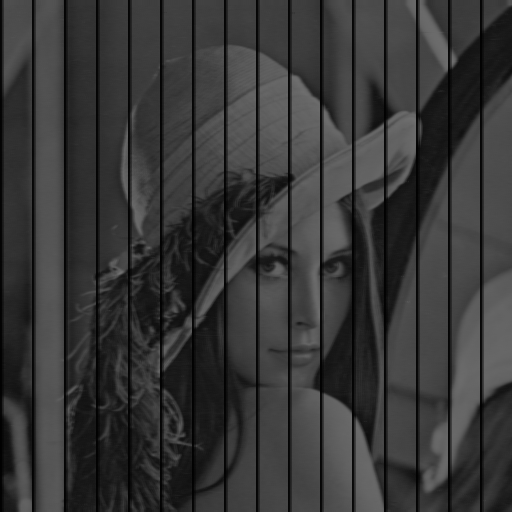
\includegraphics[scale=0.2]{../img/received_part3a.png}
\caption{Imagen Recibida}

\end{figure}

\begin{figure}[H]
\centering
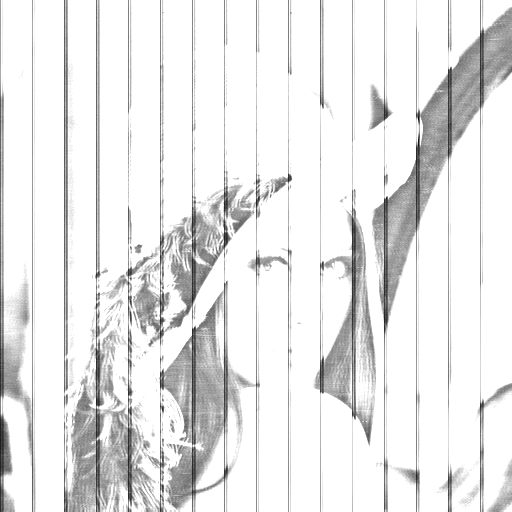
\includegraphics[scale=0.2]{../img/corrected_part3a.png}
\caption{Imagen Recuperada}

\end{figure}



\par \large{Suponiendo L=3.}
\par El error al estimar h fue:\\ 
\par   2.21210531670124e-06
\par   2.23888955847018e-06
\par   2.46672604342635e-07
\par   1.50809537170849e-01
\par   1.70955645505803e-01\\


\begin{figure}[H]
\centering
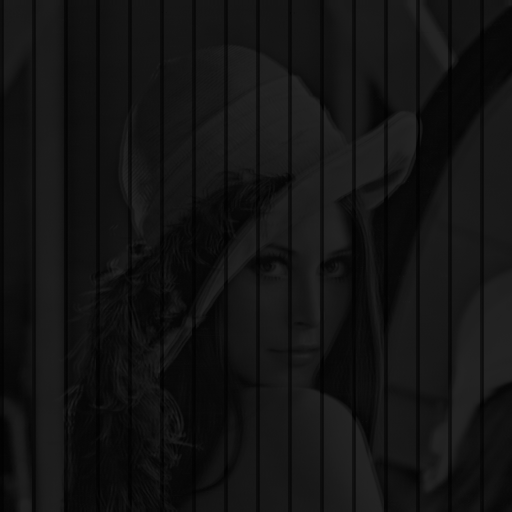
\includegraphics[scale=0.2]{../img/received_part3b.png}
\caption{Imagen Recibida}

\end{figure}

\begin{figure}[H]
\centering
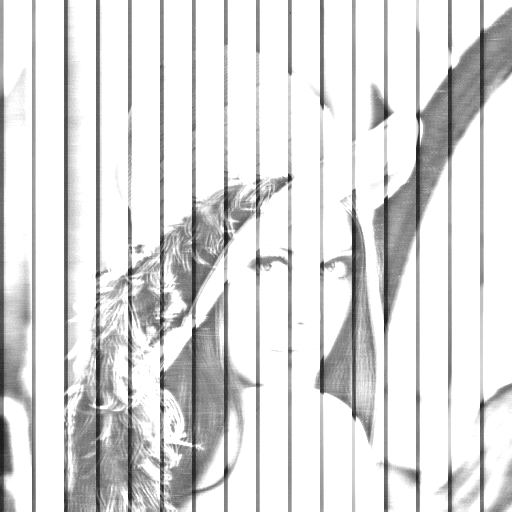
\includegraphics[scale=0.2]{../img/corrected_part3b.png}
\caption{Imagen Recuperada}

\end{figure}




\par \large{Suponiendo L=5.}
\par El error al estimar h fue:\\ 
\par   2.82588050182220e-07
\par   1.32275305559093e-05
\par   1.96310588279625e-06
\par   4.62617064481835e-06
\par   5.62121598386700e-07\\


\begin{figure}[H]
\centering
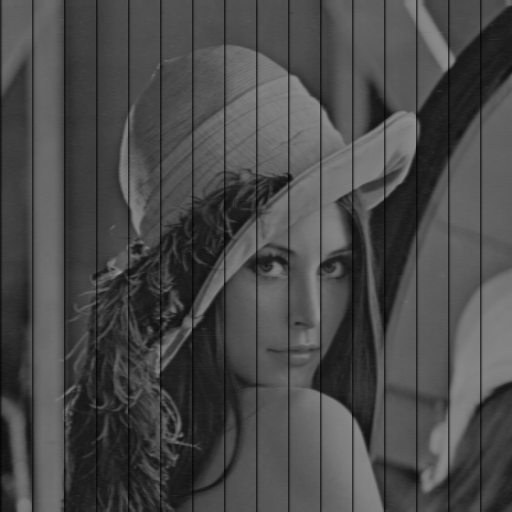
\includegraphics[scale=0.2]{../img/received_part3c.png}
\caption{Imagen Recibida}

\end{figure}

\begin{figure}[H]
\centering
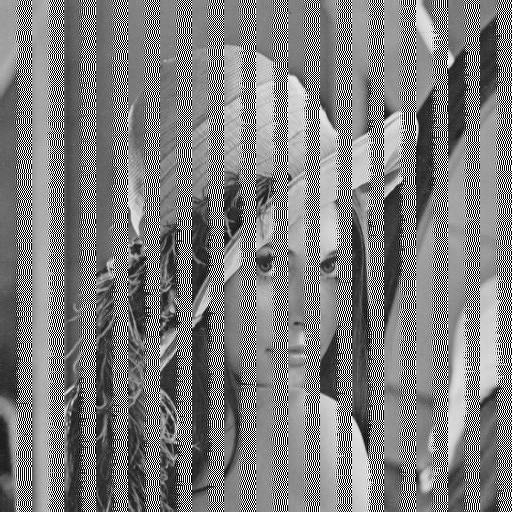
\includegraphics[scale=0.2]{../img/corrected_part3c.png}
\caption{Imagen Recuperada}

\end{figure}



\textbf{\large E = 32,  $\sigma$ = 0.01  }\\

\par \large{Suponiendo L=1.}
\par El error al estimar h fue:\\ 
\par   5.57204903386954e-06
\par   8.94206341063025e-02
\par   6.96736749314932e-03
\par   1.31128977056077e-01
\par   7.29150556624208e-02\\


\begin{figure}[H]
\centering
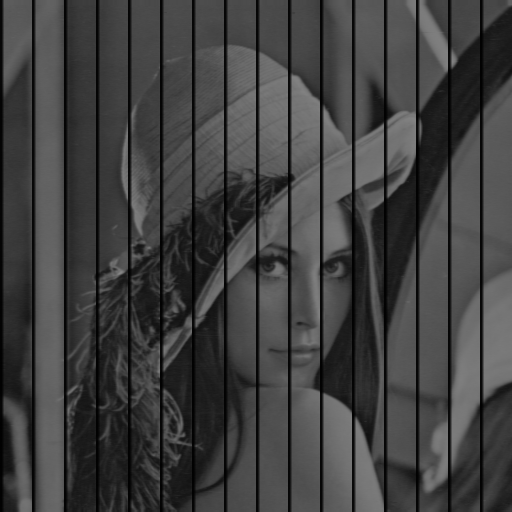
\includegraphics[scale=0.2]{../img/received_part4a.png}
\caption{Imagen Recibida}

\end{figure}

\begin{figure}[H]
\centering

\includegraphics[scale=0.2]{../img/corrected_part4a.png}
\caption{Imagen Recuperada}

\end{figure}



\par \large{Suponiendo L=3.}
\par El error al estimar h fue:\\ 
\par   1.97271398003074e-06
\par   1.56387741185871e-05
\par   1.05949822686788e-05
\par   8.36945405055923e-02
\par   3.36241020002239e-02\\

\begin{figure}[H]
\centering
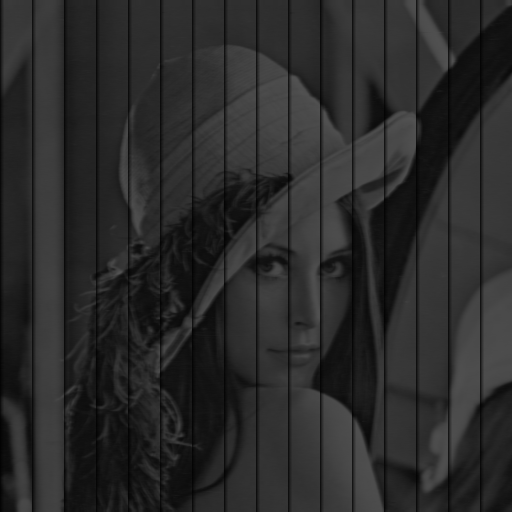
\includegraphics[scale=0.2]{../img/received_part4b.png}
\caption{Imagen Recibida}

\end{figure}

\begin{figure}[H]
\centering
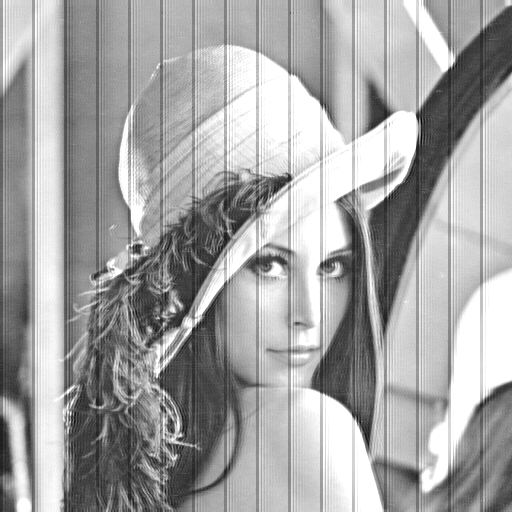
\includegraphics[scale=0.2]{../img/corrected_part4b.png}
\caption{Imagen Recuperada}

\end{figure}




\par \large{Suponiendo L=5.}
\par El error al estimar h fue:\\ 
\par   6.09505131402011e-06
\par   2.79206028110310e-05
\par   3.93434730151798e-05
\par   3.38890748193821e-05
\par   2.85690816251571e-05\\

\begin{figure}[H]
\centering
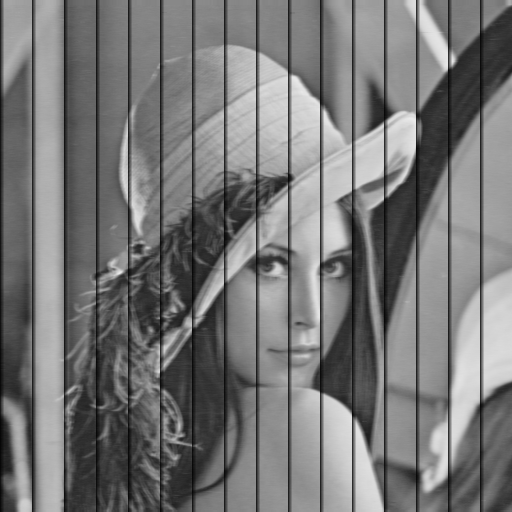
\includegraphics[scale=0.2]{../img/received_part4c.png}
\caption{Imagen Recibida}

\end{figure}

\begin{figure}[H]
\centering
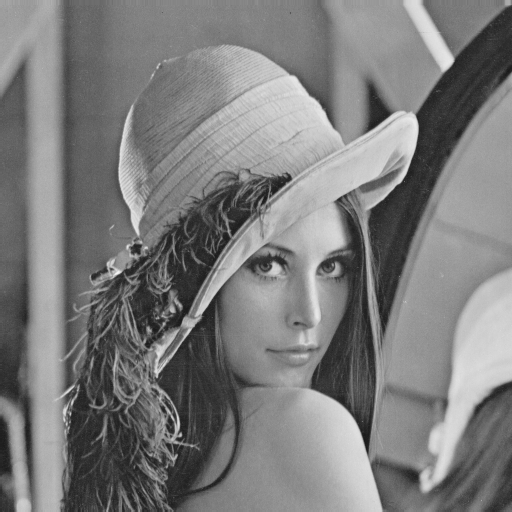
\includegraphics[scale=0.2]{../img/corrected_part4c.png}
\caption{Imagen Recuperada}

\end{figure}



\textbf{\large E = 1024,  $\sigma$ = 0.01 }\\

\par \large{Suponiendo L=1.}
\par El error al estimar h fue:\\ 
\par   7.41564685047269e-07
\par  1.22306742447753e-01
\par   2.84237281719386e-01
\par   6.17325936170009e-02
\par   1.54787518630523e-03\\


\begin{figure}[H]
\centering
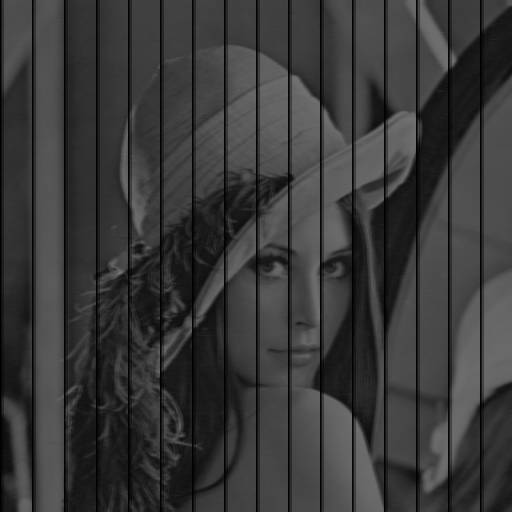
\includegraphics[scale=0.2]{../img/received_part5a.png}
\caption{Imagen Recibida}

\end{figure}

\begin{figure}[H]
\centering

\includegraphics[scale=0.2]{../img/corrected_part5a.png}
\caption{Imagen Recuperada}

\end{figure}



\par \large{Suponiendo L=3.}

\par El error al estimar h fue:\\ 
\par   3.89915389698015e-07
\par   2.04317964785927e-06
\par   1.39987199031244e-06
\par   1.58869179782212e-01
\par   2.67648902523867e-03\\

\begin{figure}[H]
\centering
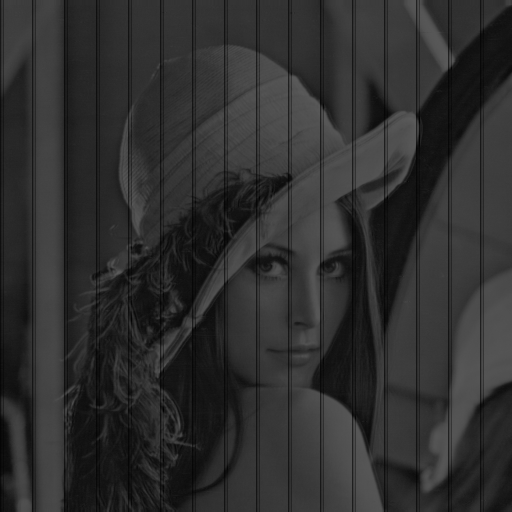
\includegraphics[scale=0.2]{../img/received_part5b.png}
\caption{Imagen Recibida}

\end{figure}

\begin{figure}[H]
\centering
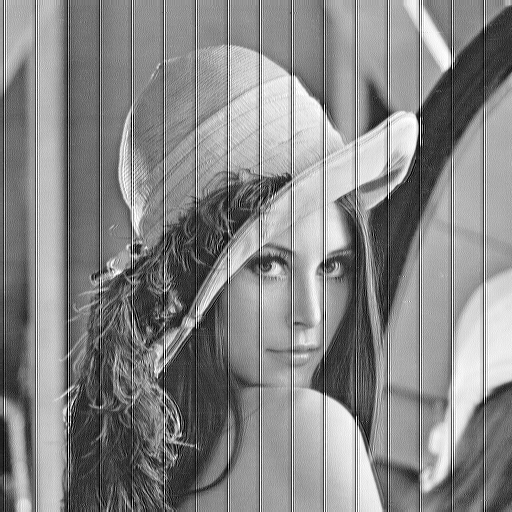
\includegraphics[scale=0.2]{../img/corrected_part5b.png}
\caption{Imagen Recuperada}

\end{figure}





\par \large{Suponiendo L=5.}

\par El error al estimar h fue:\\ 
\par   8.57149750378705e-07
\par   5.07209018510424e-06
\par   2.00696787977517e-06
\par   3.09745779877857e-06
\par   6.08170666729912e-07\\



\begin{figure}[H]
\centering
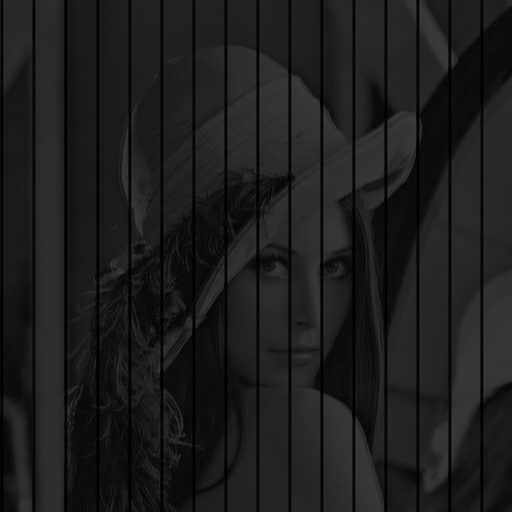
\includegraphics[scale=0.2]{../img/received_part5c.png}
\caption{Imagen Recibida}

\end{figure}

\begin{figure}[H]
\centering
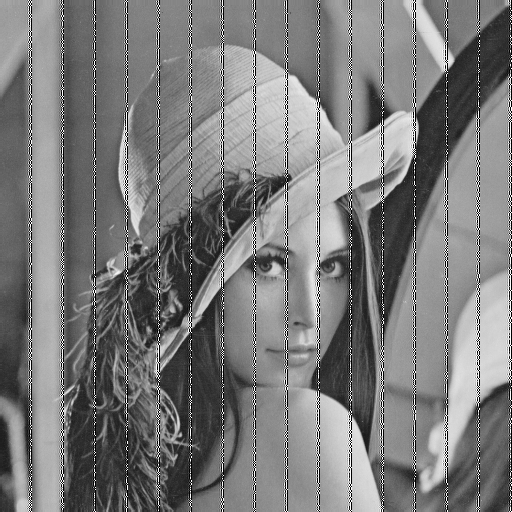
\includegraphics[scale=0.2]{../img/corrected_part5c.png}
\caption{Imagen Recuperada}

\end{figure}




\textbf{\large E = 512,  $\sigma$ = 0 }\\




\par \large{Suponiendo L=1.}
\par El error al estimar h fue:\\ 
\par   6.93889390390723e-18
\par   1.87016036254111e-01
\par   1.05858977334859e-01
\par   2.67652018807568e-01
\par   1.40969371525189e-01\\


\begin{figure}[H]
\centering
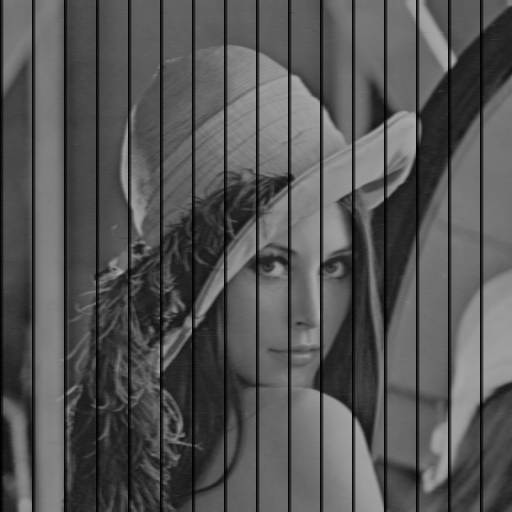
\includegraphics[scale=0.2]{../img/received_part6_3a.png}
\caption{Imagen Recibida}

\end{figure}

\begin{figure}[H]
\centering

\includegraphics[scale=0.2]{../img/corrected_part6_3a.png}
\caption{Imagen Recuperada}

\end{figure}



\par \large{Suponiendo L=3.}

\par El error al estimar h fue:\\ 
\par   9.85322934354826e-16
\par   1.38777878078145e-17
\par   9.71445146547012e-16
\par   6.02180470483583e-02
\par   2.54199365682852e-01\\

\begin{figure}[H]
\centering
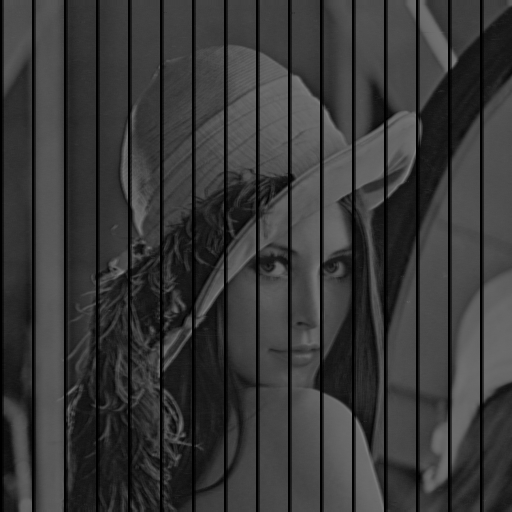
\includegraphics[scale=0.2]{../img/received_part6_3b.png}
\caption{Imagen Recibida}

\end{figure}

\begin{figure}[H]
\centering
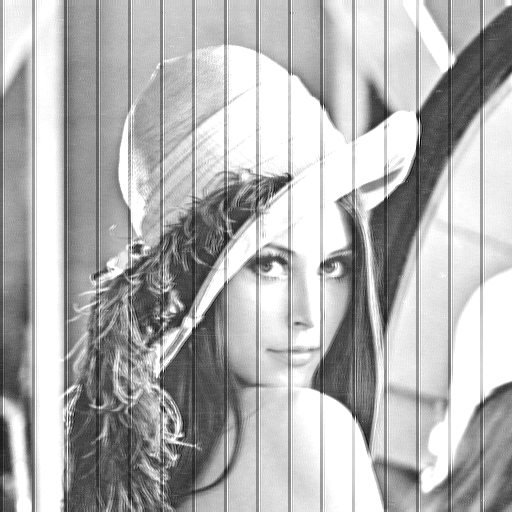
\includegraphics[scale=0.2]{../img/corrected_part6_3b.png}
\caption{Imagen Recuperada}

\end{figure}


\par \large{Suponiendo L=5.}

\par El error al estimar h fue:\\ 
\par   1.20736753927986e-15
\par   1.87350135405495e-16
\par   2.29330443524134e-15
\par   3.19189119579733e-16
\par   8.88178419700125e-16\\

\begin{figure}[H]
\centering
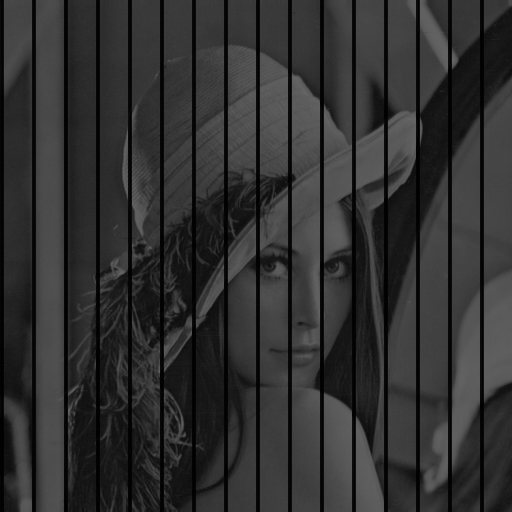
\includegraphics[scale=0.2]{../img/received_part6_3c.png}
\caption{Imagen Recibida}

\end{figure}

\begin{figure}[H]
\centering
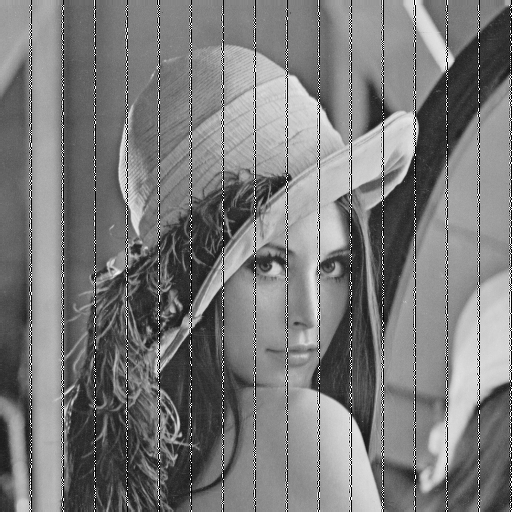
\includegraphics[scale=0.2]{../img/corrected_part6_3c.png}
\caption{Imagen Recuperada}

\end{figure}

\textbf{\large E = 512,  $\sigma$ = 0.1 }\\




\par \large{Suponiendo L=5.}
\par El error al estimar h fue:\\ 
\par   2.77818408822572e-06
\par   6.39480579725515e-07
\par   8.56564309231755e-07
\par   1.47781988831669e-05
\par   4.98113753122191e-06


\begin{figure}[H]
\centering
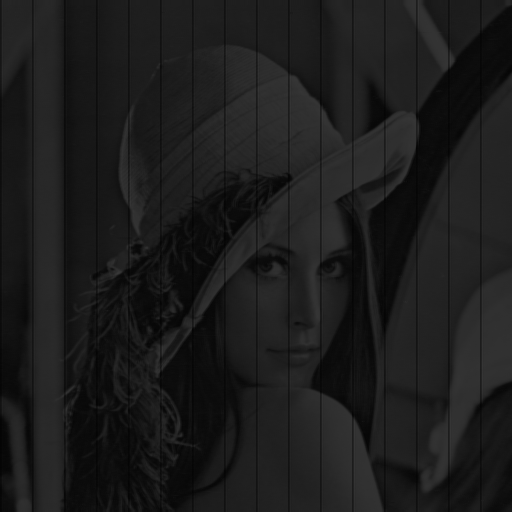
\includegraphics[scale=0.2]{../img/received_BONUS.png}
\caption{Imagen Recibida}

\end{figure}

\begin{figure}[H]
\centering
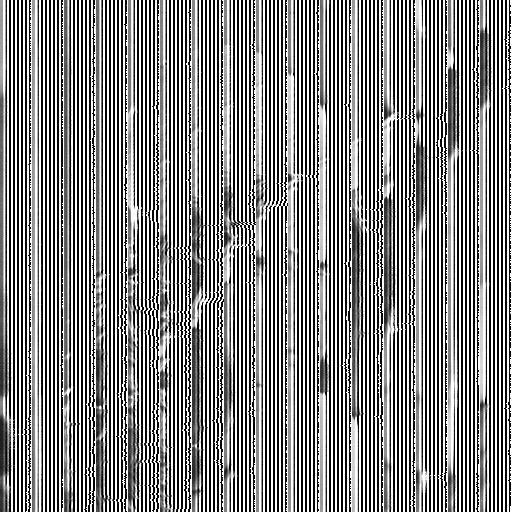
\includegraphics[scale=0.2]{../img/corrected_BONUS.png}
\caption{Imagen Recuperada}

\end{figure}




\section{Conclusiones}

\par Como se mencionó anteriormente, las imagenes recibidas nunca permanecen iguales a las que fueron enviadas, puesto que se reinterpreta el mensaje con una estimación de la respuesta al impulso del canal real y además, es imposible contrarrestar el efecto del ruido blanco Gaussiano. Sin embargo, modificando ciertos parametros en el proceso de reinterpretación del mensaje, en particular E, L, y sigma; es posible obtener una peor o una mejor aproximación al mensaje original transmitido. Es evidente que cuanto menor sea el error de estimación, menos se va a ver alterada la imagen reconstruida. 
\par El primer parámetro a analizar es L, es decir, la longitud de la respuesta al impulso. Como el L real es 5, es lógico que al suponer un Lguess menor, se esté estimando un h menos exacto. Esto se debe que al realizar las pruebas con un Lguess menor a 5, se estiman los primeros "Lguess" valores de h real, por lo que el error se mantiene en un valor esperado en estos valores de h (orden menor a -6), pero los h que no fueron estimados, permanecen en 0. Esto provoca que el al recuperar la imagen, estos h que no fueron estimados interfieran en la correcta reinterpretacion de la imagen. En consecuencia, como se puede observar en los Resultados, a medida que el Lguess que se supone se acerca al L real, el error disminuye y la semejanza entre la imagen recibida y la recuperada es superior. Es más, suponiendo un L=x, si se observa el vector del error en la estimacion, los primeros x valores son coherentes con un error, mientras los demás  no.
\par El parametro E tiene que ver con la longitud del mensaje conocido que se usa para estimar h, es decir, el mensaje que se somete a la secuencia de "entrenamiento". Tal como se nota en los resultados, cuanto mas se "entrena" la cadena, el error es menor, y asi la estimacion del h es mejor. Analizando en un mismo L distintos E, se puede observar como mejora el error cuando E es mas grande.
\par Por último, $\sigma$. Este parámetro hace referencia a la desviación típica del random con distribución normal que establece el ruido blanco Gaussiano. Notar que cuando sigma es 0, el error en los valores de h estimados bajan al orden de -16, es decir, sin ruido, la esitmación es casi exacta.  Evidentemente, si la perturbación por el ruido blanco Gaussiano es menor, la tarea de reinterpretación se facilita, pues, como se dijo antes, esta perturbación es imposible de tener en cuenta en el proceso para recuperar el mensaje.
\par Se puede apreciar que la mejor aproximación y la mejor recuperacón de la imagen se obtiene cuando se reúnen casi todos los requisitos óptimos de los tres parámetros(a pesar del E que podría ser 1024), L=5, E=512 y $\sigma$=0.



\end{multicols}


\clearpage

\section{Anexo}
\par Aquí se pueden ver las funciones de \textit{GNU Octave} utilizadas para este análisis.\\

\par El \textit{script} \verb+initializeCannal.m+ inicializa las variables del canal.

\begin{ttfamily}
\begin{center}
\fbox{\parbox{6in}{\textbf{initializeCannal.m} \\
\verbatiminput{../src/initializeCannal.m}}}
\end{center}
\end{ttfamily}

\par El \textit{script} \verb+simulation.m+ implementa la simulacion del sistema de comunicacion .

\begin{ttfamily}
\begin{center}
\fbox{\parbox{6in}{\textbf{simulation.m} \\
\verbatiminput{../src/simulation.m}}}
\end{center}
\end{ttfamily}

\par El \textit{script} \verb+train.m+ implementa la secuencia de entrenamiento.

\begin{ttfamily}
\begin{center}
\fbox{\parbox{6in}{\textbf{train.m} \\
\verbatiminput{../src/train.m}}}
\end{center}
\end{ttfamily}

\par El \textit{script} \verb+transmit.m+ simula la transmicion por el canal.

\begin{ttfamily}
\begin{center}
\fbox{\parbox{6in}{\textbf{transmit.m} \\
\verbatiminput{../src/transmit.m}}}
\end{center}
\end{ttfamily}

\par El \textit{script} \verb+cholesky.m+ obtiene la descomposición de Cholesky de una matriz simétrica.

\begin{ttfamily}
\begin{center}
\fbox{\parbox{6in}{\textbf{cholesky.m} \\
\verbatiminput{../src/cholesky.m}}}
\end{center}
\end{ttfamily}

\par El \textit{script} \verb+minimumSquares.m+ resuelve los cuadrados mínimos por Cholesky.

\begin{ttfamily}
\begin{center}
\fbox{\parbox{6in}{\textbf{minimumSquares.m} \\
\verbatiminput{../src/minimumSquares.m}}}
\end{center}
\end{ttfamily}

\par El \textit{script} \verb+backSustitution.m+ hace la sustitucion hacia atras.

\begin{ttfamily}
\begin{center}
\fbox{\parbox{6in}{\textbf{backSustitution.m} \\
\verbatiminput{../src/backSustitution.m}}}
\end{center}
\end{ttfamily}


\par El \textit{script} \verb+saveImages.m+ guarda las imagenes.

\begin{ttfamily}
\begin{center}
\fbox{\parbox{6in}{\textbf{saveImages.m} \\
\verbatiminput{../src/saveImages.m}}}
\end{center}
\end{ttfamily}

\par El \textit{script} \verb+calculatehError.m+ calcula el error de h.

\begin{ttfamily}
\begin{center}
\fbox{\parbox{6in}{\textbf{calculatehError.m} \\
\verbatiminput{../src/calculatehError.m}}}
\end{center}
\end{ttfamily}


\par El \textit{script} \verb+estimateh.m+ estima el valor de h.

\begin{ttfamily}
\begin{center}
\fbox{\parbox{6in}{\textbf{estimateh.m} \\
\verbatiminput{../src/estimateh.m}}}
\end{center}
\end{ttfamily}

\end{document}
